\sisetup{locale = EN} 
\begin{document}\selectlanguage{english}
\section*{Tracking}
\begin{figure}[h]
     \begin{minipage}[t]{0.6\textwidth}
      \vspace{-6cm} Wir kennen den Aufbau des LHCb-Experiments am CERN aus dem Einführungsvortrag. Nun wollen wir die Informationen nutzen und die Masse von Teilchen abschätzen, die wir mit dem Detektor direkt messen können. Aus diesen Massen kann anschließend die Masse des Mutterteilchens rekonstruiert werden, das werden wir heute Nachmittag sehen! 
      
      Wir nehmen den Detektor als zweidimensional an, sowie dass die Kalorimeter die Energie sehr exakt bestimmen können (s. Abb. \ref{fig: Der Detektor}). Dies hat den Vorteil, dass die RICH-Subdetektoren vernachlässigt werden können. Der Magnet wird als homogen mit einer magnetischen Flussdichte von B$\,=\,$0.4\,T angenommen.  Konstanten: Vakuumlichtgeschwindigkeit $c~=~ 299792458 \, \nicefrac{m}{s}$; Elementarladung $e~=~ 1.602176634\cdot10^{-19}$\,C.  \end{minipage}
            \begin{minipage}[t]{0.4\textwidth}
            \centering
            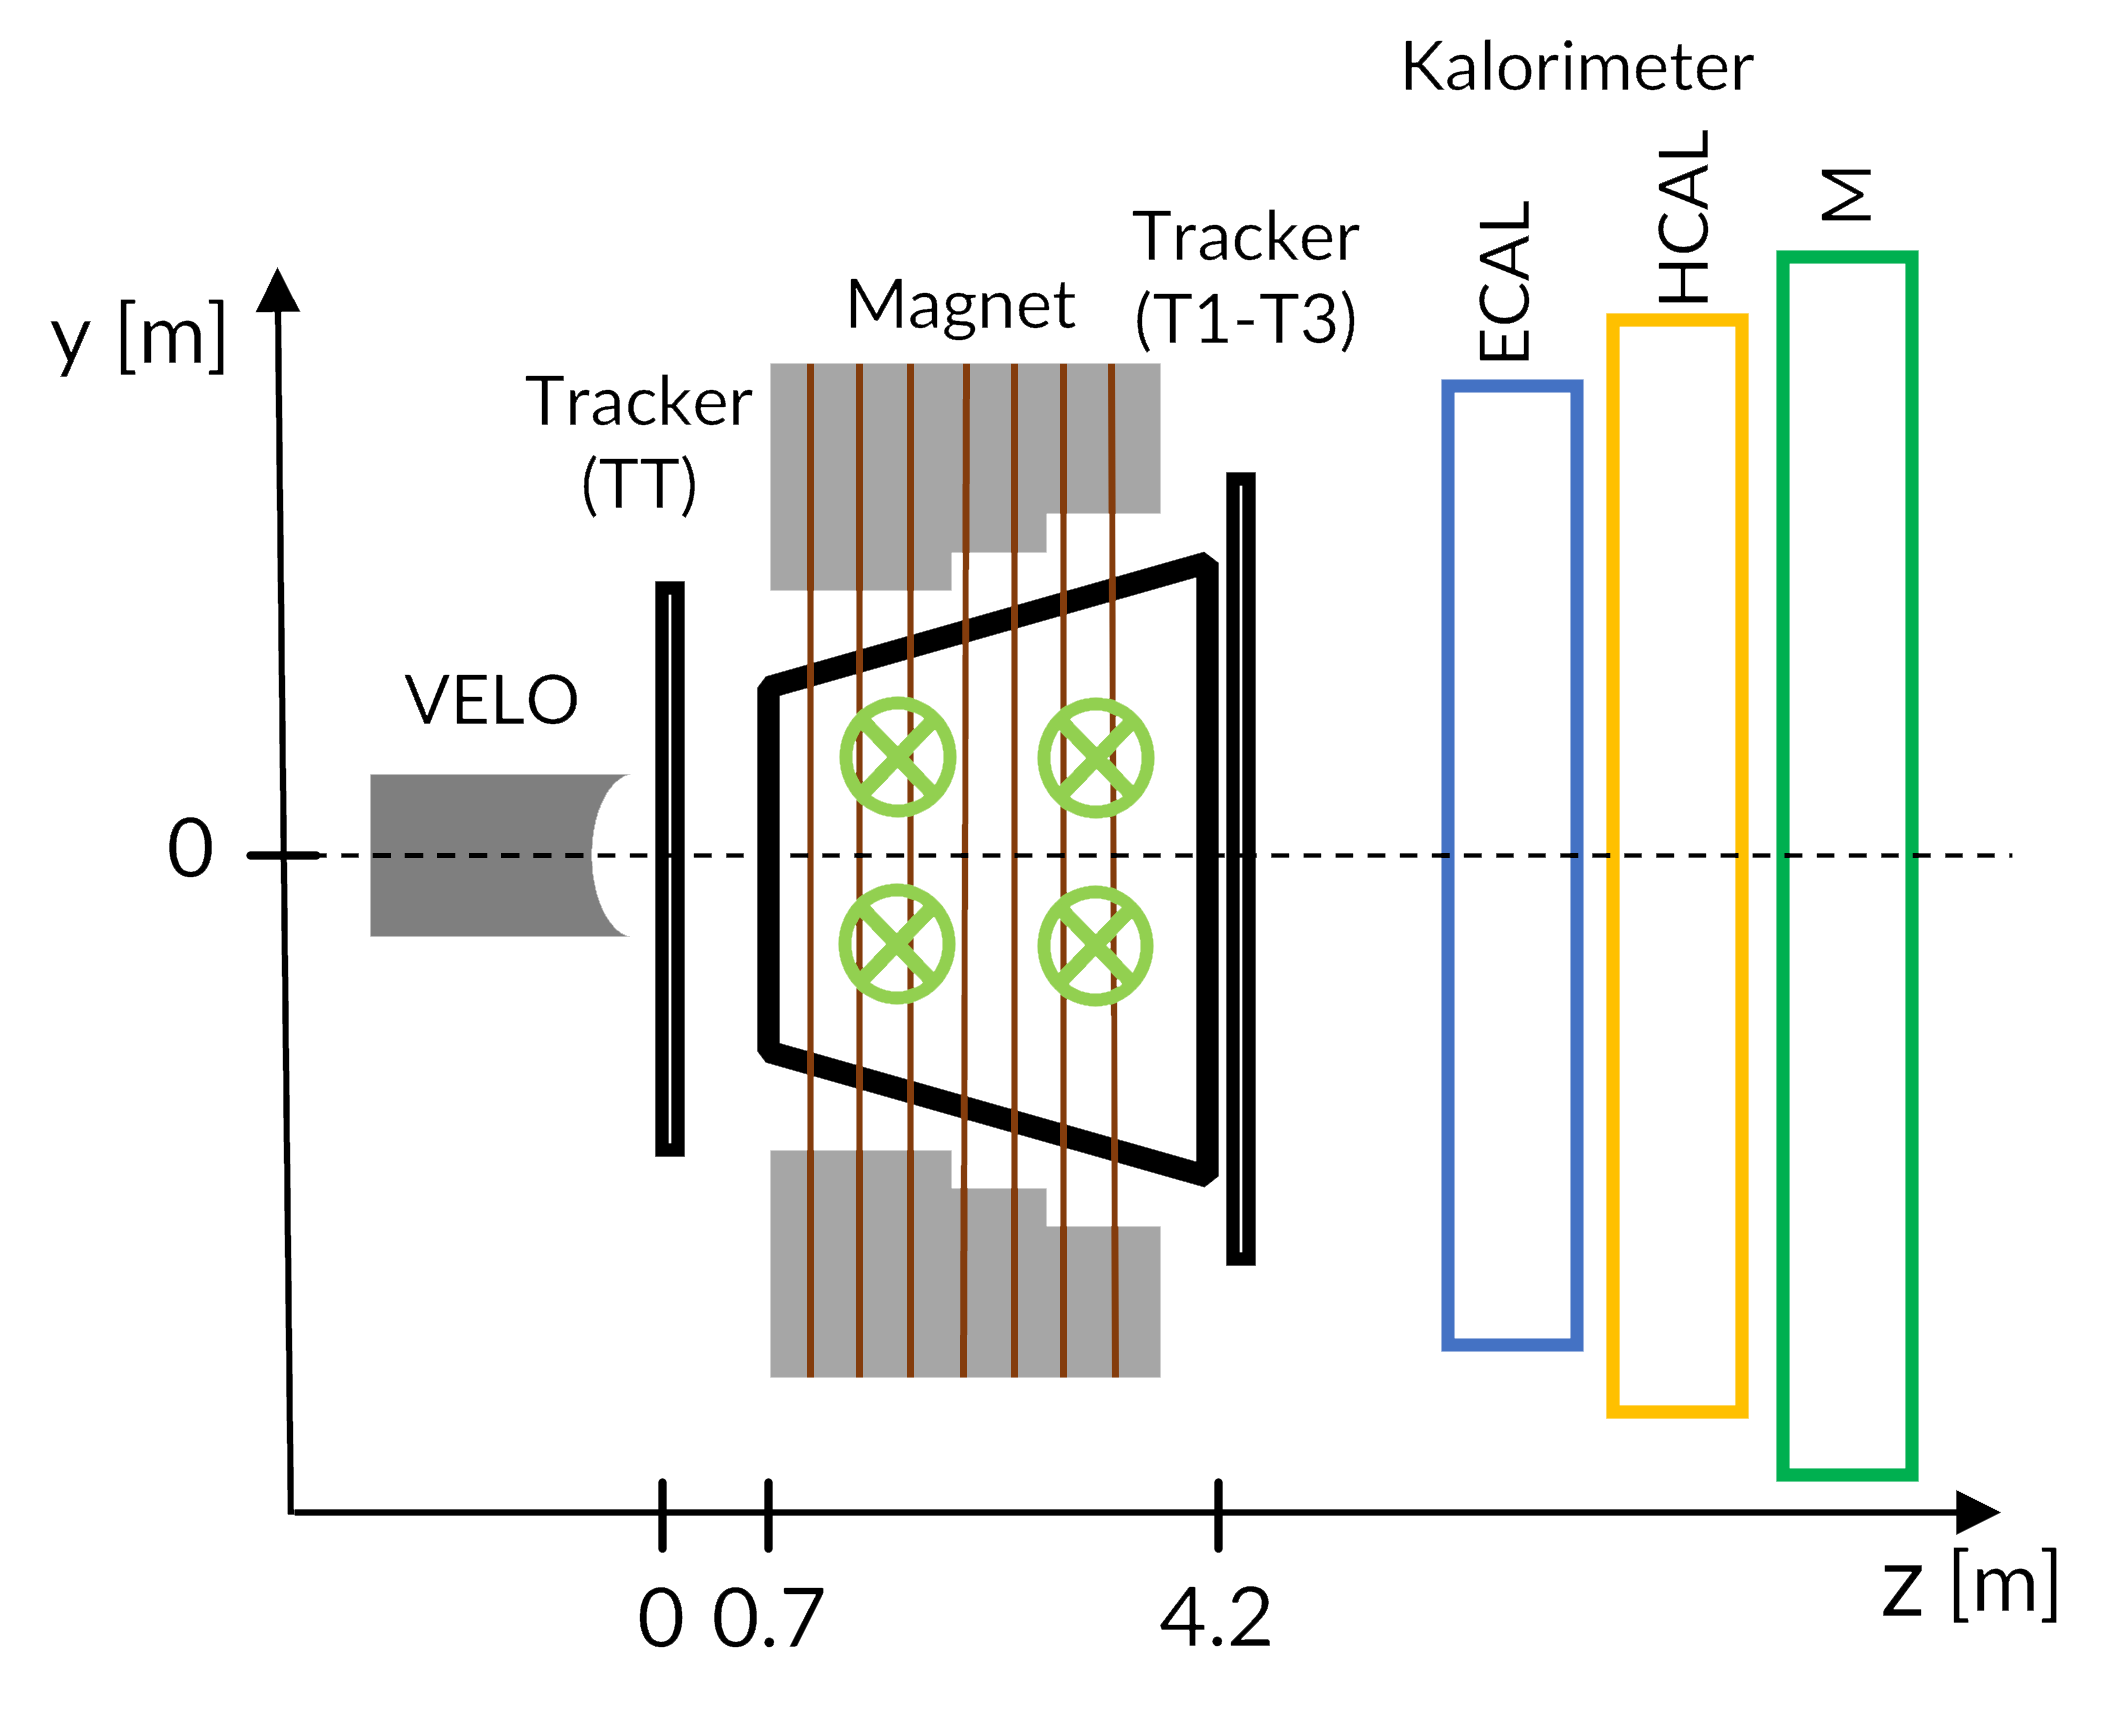
\includegraphics[width=\textwidth]{Figures Worksheets/LHCb_Calculation_LHCb_Detector_DE.png} 
            \caption{Vereinfachter LHCb-Detektor} \label{fig: Der Detektor}
            \end{minipage}
            \end{figure}
\subsection*{Messdaten}
Die nachstehende Tabelle beinhaltet die Daten eines Zerfalls, welcher das Triggersystem aktiviert und als womöglich spannend identifiziert hat. Außerdem sehen Sie einen Ausschnitt des Vertex Locators (VELO), welcher sich um den Kollisionspunkt befindet. Dort interagieren die Reaktionsprodukte mit hintereinander angeordneten Siliciummodulen  (grün), sodass sich Spuren und Ursprungspunkte sekundärer Zerfälle identifizieren lassen.
\begin{figure}[h]
    \centering
   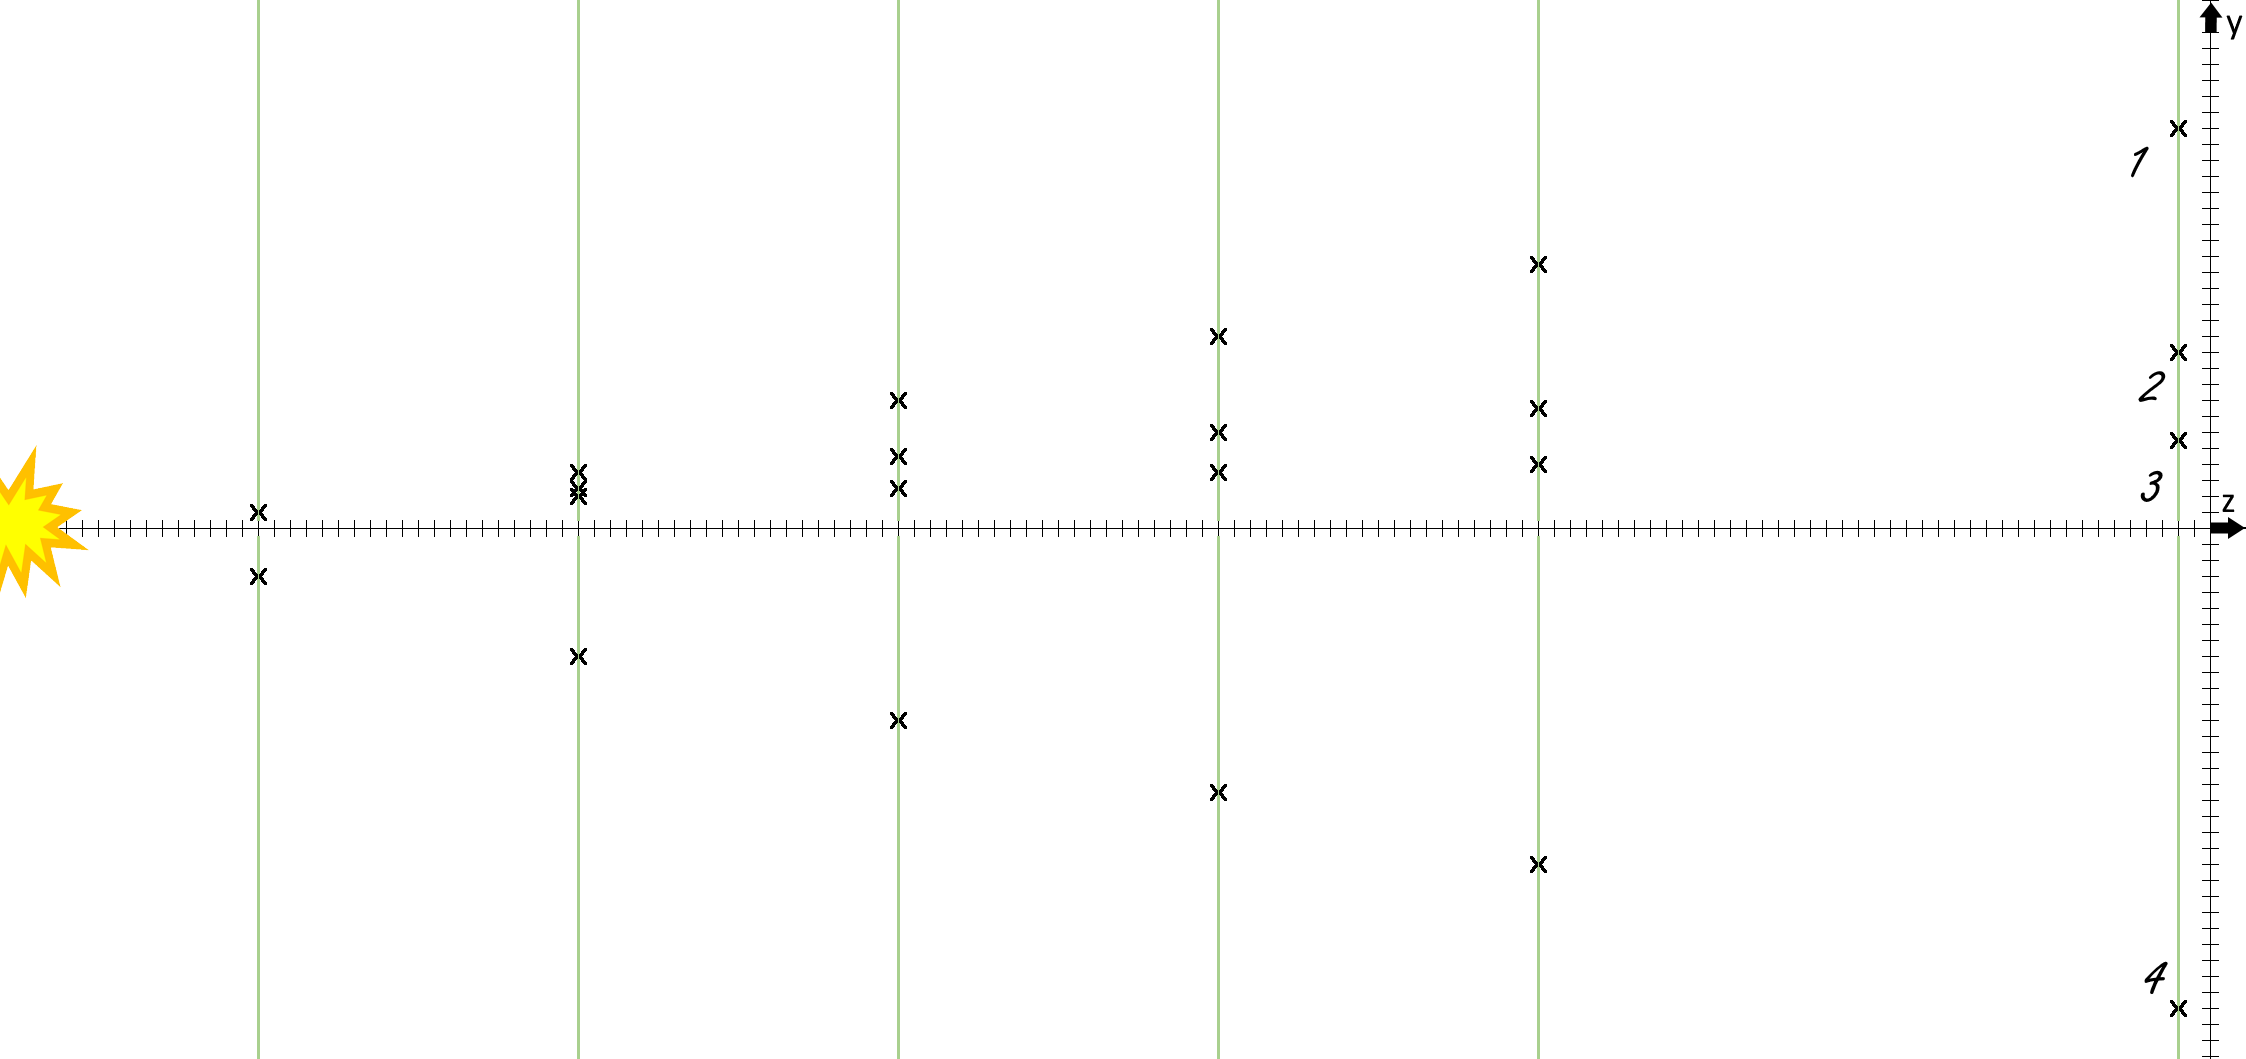
\includegraphics[width=\textwidth]{Figures Worksheets/LHCb_Calculation Task.png}\label{fig: VELO}
   \caption{Seitliche Ansicht der Ereignisse an den Siliciummodulen (grün) des VELOs, welcher um den Kollisionspunkt angeordnet ist. Hieraus lassen sich Ursprungsorte von weiteren Zerfällen und Winkel von Spuren relativ zur $z$-Achse bestimmen.}
\end{figure}
\begin{table}
\centering
 \caption{Datentabelle über das Ereignis. Angegeben für die Spuren die Orte im Trackersystem vor (TT) und nach (T1-T3) dem Magnetfeld. Die im Elektromagnetischen Kaloriemeter (ECAL) deponierte Energie sowie die im Hadronischen Kaloriemeter (HCAL) sind zu einer Gesamtenergie verrechnet worden. Außerdem die Angabe, ob das Myonensystem (M) getriggert wurde.}
\begin{tabular}{|c||r|r|r|r|r|c|}

\hline
\rowcolor{LHCbDarkBlue} \T\B \textcolor{LHCbLightBlue}{Spur} & \textcolor{LHCbLightBlue}{$y_{TT}$} & \textcolor{LHCbLightBlue}{$y_{T1-T3}$} & \textcolor{LHCbLightBlue}{$E_{ECAL}$} & \textcolor{LHCbLightBlue}{$E_{HCAL}$}& \textcolor{LHCbLightBlue}{$E_{ges}$} & \textcolor{LHCbLightBlue}{M}  \\
\hline\rowcolor{LHCbLightBlue}\T\B  & m & m & GeV & GeV& GeV & \\
\hline\hline 
\T\B 1 & 0.72769 & 2.89240 & 0.0461& 0.3727& 0.4188&Leer\\ 
\T\B 2 & 0.30505 & 0.83866 & 0.4902 & 3.9661 &4.4563& Leer\\
\T\B 3 & 0.12215 & -0.02320 & 0.3072 & 2.2530 &2.5602& Leer \\ 
\T\B 4 & -0.78733 & -1.93223 & 0.4791 & 3.5142 & 3.9933&Leer \\  


\hline
\end{tabular}\end{table}\\ \, \\ 
%\kariert{Platz für Notizen und Zeichnungen}{16}{14}






\SetDefinition{\textbf{Aufgabe:} Öffnen und starten Sie den vor Ihnen stehenden PC. Hier finden Sie Aufgaben, die Sie mit den Abbildungen und Tabellen auf diesem Arbeitsblatt durchführen können. \\ \emph{Sie werden dort etwas programmieren, die Eingaben unterscheiden sich zu gewohnten Schreibweisen entsprechend der unterstehenden Tabelle. Falls Sie Schwierigkeiten haben, sprechen Sie uns an! }}



\textbf{\sffamily Hinweise zum selbstständigen Programmieren}
\begin{table}[h]
    \centering
    \begin{tabular}{c|c}
       Gewohnter Ausdruck  & Schreibweise in Jupyter Notebook \\ \hline
       $1,0$&$1.0$\\
       $a+b$&$a+b$\\
        $a-b$&$a-b$\\
       $a\cdot b $& $a*b$ \\
       $a:b$ & $a/b$ \\
       $a^b$  & $a**b$ \\
       $\sqrt{a}$&$a**0.5$
       
       
    \end{tabular}

\end{table}

\kariert{Hier Platz für Notizen}{16}{4}
\end{document}